\section{BÚSQUEDA APROXIMADA DE VECINOS CERCANOS}

La \textit{Búsqueda Aproximada de Vecinos Cercanos (ANN)} es una de las propuestas más avanzadas de optimización para los enfoques \textit{k-NN} redefiniendo el objetivo principal para obtener resultados con tasa de efectividad similar pero con un costo computacional más bajo.

\begin{definition}
    Sea $d_k$ la distancia del \textbf{verdadero} k-ésimo vecino más cercano, el algoritmo \textit{ANN} devuelve un vecino cuya distancia $d'$ cumple con: 
    \begin{equation}
        d' \leq (1 + \epsilon) \cdot d_k
        \addequation{Grado de Tolerancia del Algoritmo de Vecinos Aproximadamente más Cercanos}
    \end{equation}
    Donde $(1 + \epsilon)$ representa el grado de proximidad respecto a los vecinos cercanos, por lo tanto, si $\epsilon = 0$ entonces nos referimos al método \textit{k-NN} debido a que no existe tolerancia de proximidad y, por el contrario, si $\epsilon = 0.1$ entonces el vecino resultante puede estar hasta $10\%$ más lejos que el verdadero k-ésimo vecino más cercano \parencite{NIPS2004_1102a326}.
\end{definition}

Este enfoque de proximidad ha sido estudiado con el fin de lograr que la \textit{Búsqueda de Vecinos Cercanos} se vuelva computacionalmente viable en sistemas de alta dimensionalidad, y gracias a estas investigaciones se han formulado diferentes metodologías y algoritmos que enfocan la proximidad de maneras diferentes. En la \Cref{fig:BenchmarkANN} se muestra una gráfica que compara el rendimiento de los algoritmos basados en \textit{ANN} según la cantidad de peticiones por segundo realizadas y la \textbf{Sensibilidad o Recall} de los resultados obtenidos. Además, a través de dicha gráfica se puede observar que existe un campo diverso de algoritmos que aprovechan este concepto, sin embargo, cada algoritmo se basa en diferentes enfoques de \textit{ANN} como \textit{Enfoques basados en hashing}, \textit{Enfoques basados en árboles} o \textit{Enfoques basados en Grafos}.

En el ámbito de los sistemas de recomendación enfocados en contenido multimedia, los enfoques más importantes de \textit{ANN} son los que están basados en árboles y grafos.

\begin{figure}[h!]
    \centering
    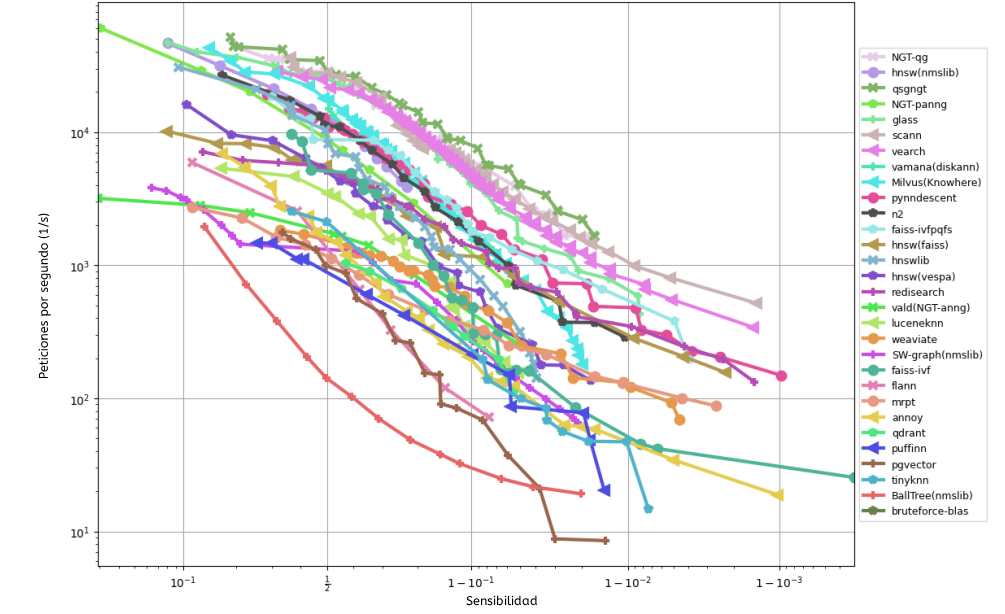
\includegraphics[width=0.9\linewidth]{BenchmarkANN.png}
    \caption{Rendimiento de los algoritmos \textit{ANN} más usados en la actualidad \parencite{20239d146dff4b27bd57f85484104308}.}
    \label{fig:BenchmarkANN} 
\end{figure}

\newpage

Según \parencite{team-2025}, los sistemas que se benefician del uso de \textit{ANN} son los que cumplen con las siguientes características:
\begin{itemize}
    \item \textbf{Conjuntos de Datos Masivos: } Es el caso de uso esencial de \textit{ANN}, de lo contrario, un enfoque de Vecinos Cercanos sería inviable.
    \item \textbf{Datos con alta dimensionalidad: } Recordando que el crecimiento de la dimensionalidad hace que la complejidad de \textit{k-NN} explote. Por lo tanto, \textit{ANN} logra reducir la dimensionalidad mediante técnicas de efectividad y optimizan el costo computacional.
    \item \textbf{Aplicaciones en Tiempo Real: } La velocidad de \textit{ANN} logra respuestas en tiempo real que sería imposible lograr con los métodos de vecinos cercanos tradicionales.
    \item \textbf{Apertura a Aproximaciones: } Si el sistema puede tolerar resultados aproximados, entonces usar \textit{ANN} es ideal para mejorar el rendimiento, de lo contrario, un enfoque de vecinos cercanos se vuelve inviable.
\end{itemize}
